\chapter{Implementation and Testing strategy}
Testing is one of the most important parts of a software development.
This phase allows to go through all the possible cases that can take place when the project goes live.
Over 75 tests have been done, only the main components have been tested.
Several external libraries are also used:
\begin{itemize}
    \item \textit{mockito}
    \item \textit{firebase\textunderscore auth\textunderscore mocks}
    \item \textit{build\textunderscore runner}
    \item \textit{fake\textunderscore cloud\textunderscore firestore}
    \item \textit{google\textunderscore sign\textunderscore in\textunderscore mocks}
    \item \textit{firebase\textunderscore storage\textunderscore mocks}
\end{itemize}






\section{Unit testing}
We used a typical stub-driver approach to test the functionalities of main components of our applications. 
\newline
\newline
\hspace*{-1cm}
\includegraphics[width=14cm,keepaspectratio]{Images/testing/stub_driver.png}
\newpage
\noindent The tested components have been
\begin{itemize}
    \item[--] FirebaseAuthHelper
    \item[--] FirestoreHelper
    \item[--] ProductsProvider
    \item[--] ShoppingListProvider
\end{itemize}

\begin{wrapfigure}{r}{0.35\textwidth}
  \begin{center}
    \vspace*{-1cm}
\includegraphics[width=0.4\textwidth]{Images/testing/logo.png}
  \end{center}
\end{wrapfigure}
To mock their dependencies and create stubs, we used \textit{Mockito}, a powerful library that helps generating stubs.
In order for those components to be testable, we had to perform a refactoring to make them compliant to testable standard structure. One of the most important thing was to be able to inject dependencies via the constructor to create stubs for internal dependencies. We managed to accomplish this by dynamically resolve ad runtime the possibility to instantiate the object with some or all its dependencies mocked.
\newline
\newline
\begin{center}
    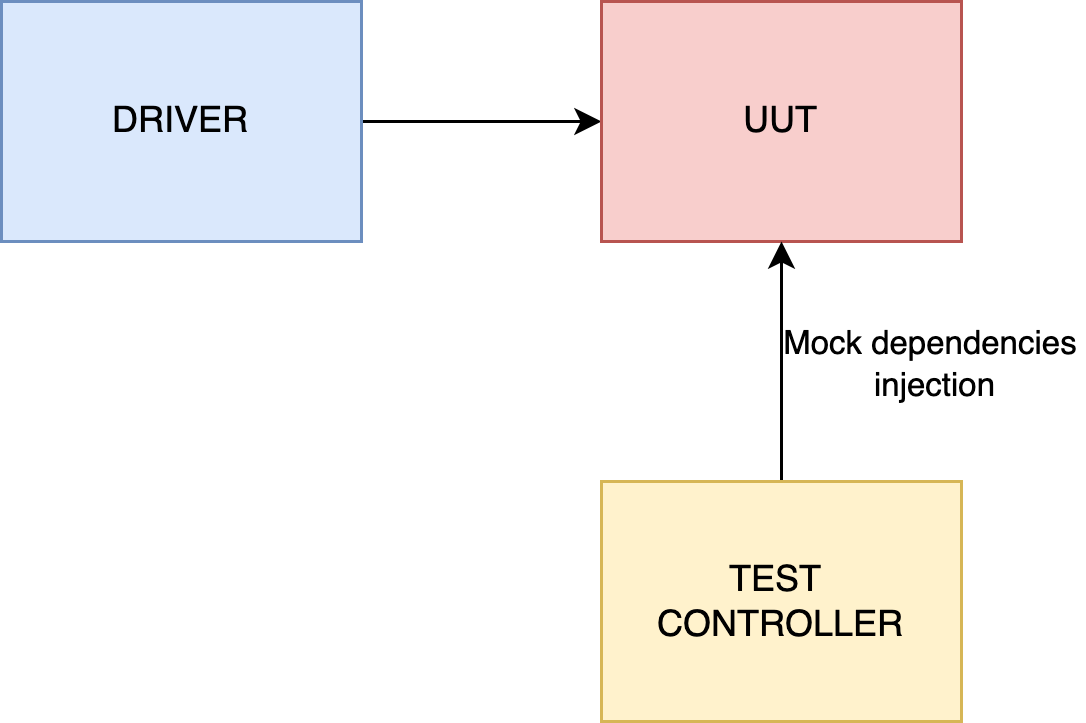
\includegraphics[width=8cm,keepaspectratio]{Images/testing/stub_driver_injection.png}
\end{center}

\noindent All of those components have been heavily tested in all of their use cases. We manage to obtain 60 tests (number also given from their complexity and dimension).
\newline
\newline
\noindent To perform assertions and evaluate tests we used the implemented flutter library called \textit{flutter\_test.dart}.

\newpage
\section{Widget testing}
Widget testing aims to test UI behavior to certain actions and it's not about functionalities and logic like the unit testing.
This type of testing is made available thanks to a \textit{Widget tester} library embedded in the flutter SDK.
\newline
\newline
\noindent The main widget tested were the sign up, sign in and the add modal product.
\newline
\newline
\noindent There it presents once again the need of using stubs because of internal dependencies inside screens and widget. The difference with the unit testing is the impossibility to perform a large scale refactoring since implementing an injectable constructor would be a tedious and very long task. We solved this by using a \textit{dependencies provider} that is responsible for providing dependencies to each widget requiring it. By doing this, each widget has dependencies fetching completely transparent while we can inject the dependencies provider with mocks to be served to widgets.

\begin{center}
    \vspace{1cm}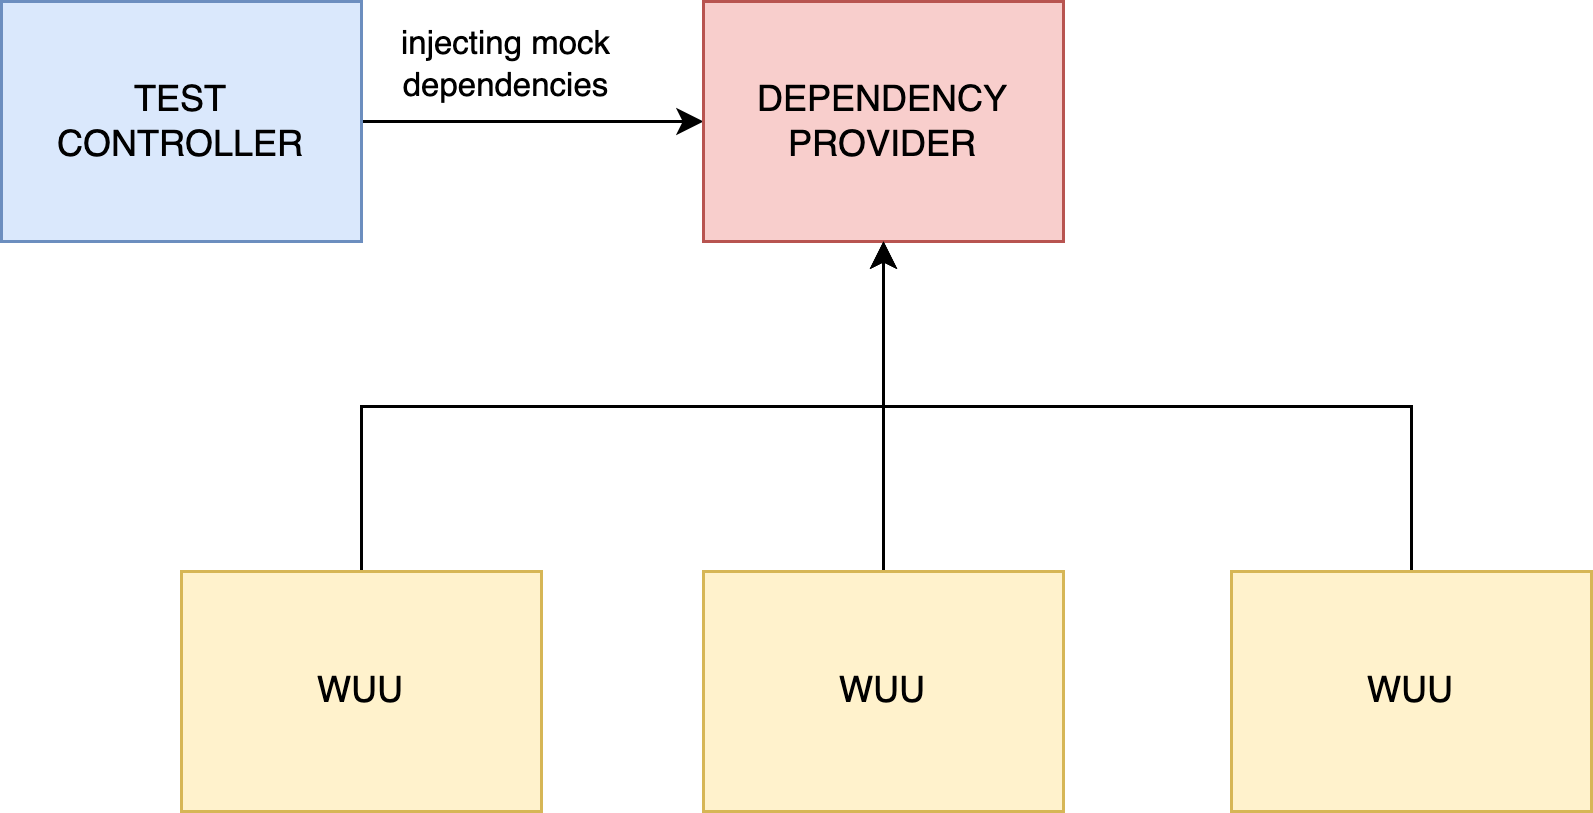
\includegraphics[width=12cm,keepaspectratio]{Images/testing/widget_testing.png}
\end{center}


\newpage
\section{Monkey testing}
Monkey testing is a technique where the user tests the application by providing random inputs and checking behaviour, or seeing whether the application or system will crash.
This test has been done using \textit{Firebase Test Lab}, that is an application-testing infrastructure offered by Google Firebase.
It permits to define different device configurations' collection on which application can be tested. Every device configuration collection works on a specific range of device types, language, and orientation configuration options.
Every test is performed via virtual and physical devices located at the Google data center.
When a test is run against devices and configurations selected, \textit{Test Lab} runs the test and display the results as a \textbf{text matrix}.
\newline
\textbf{Devices x Test Executions = Test Matrix}
\begin{figure}[H]
   \centering
  \centerline{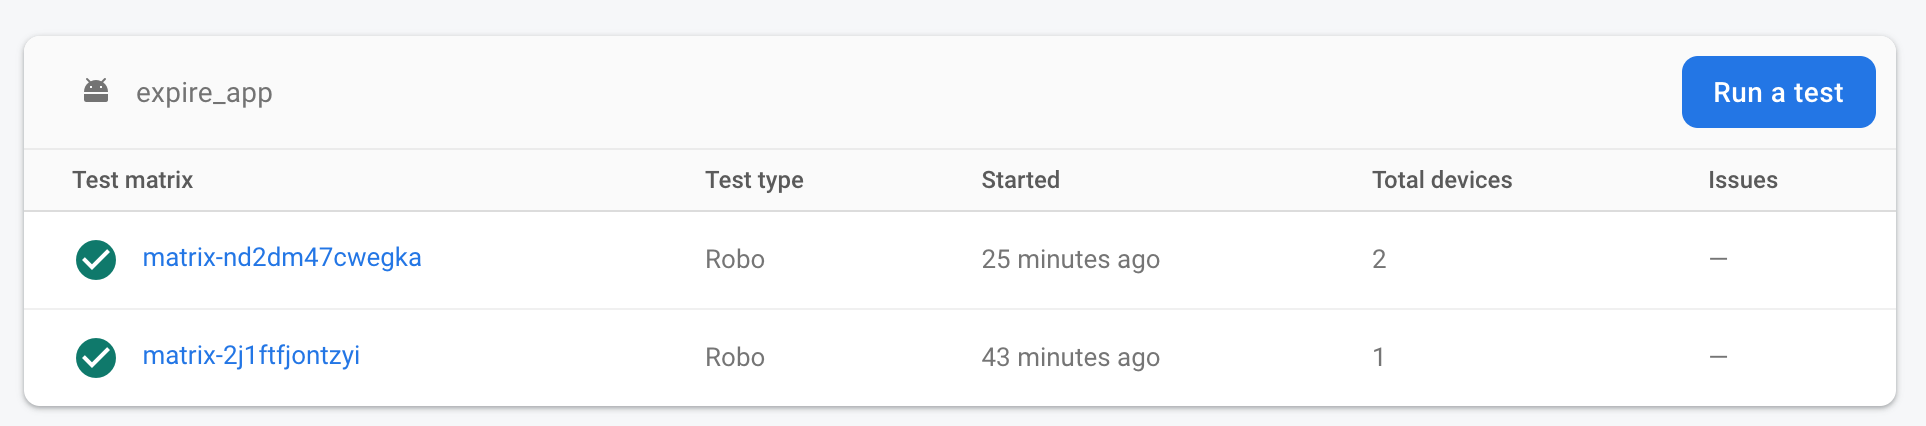
\includegraphics[width=150mm,scale=0.9]{./Images/testing/testing1.png}}
  \caption{Matrix test}
\end{figure}

Another test performed with \texit{Test Lab} is so called \textbf{robo test}.
It analyzes the structure of app's UI and explores it methodically, automatically simulating user activities.
This test captures log files, saves a series of annotated screenshots, and then creates a video form those screenshots to show the simulated operations that it performed.
\begin{figure}[H]
   \centering
  \centerline{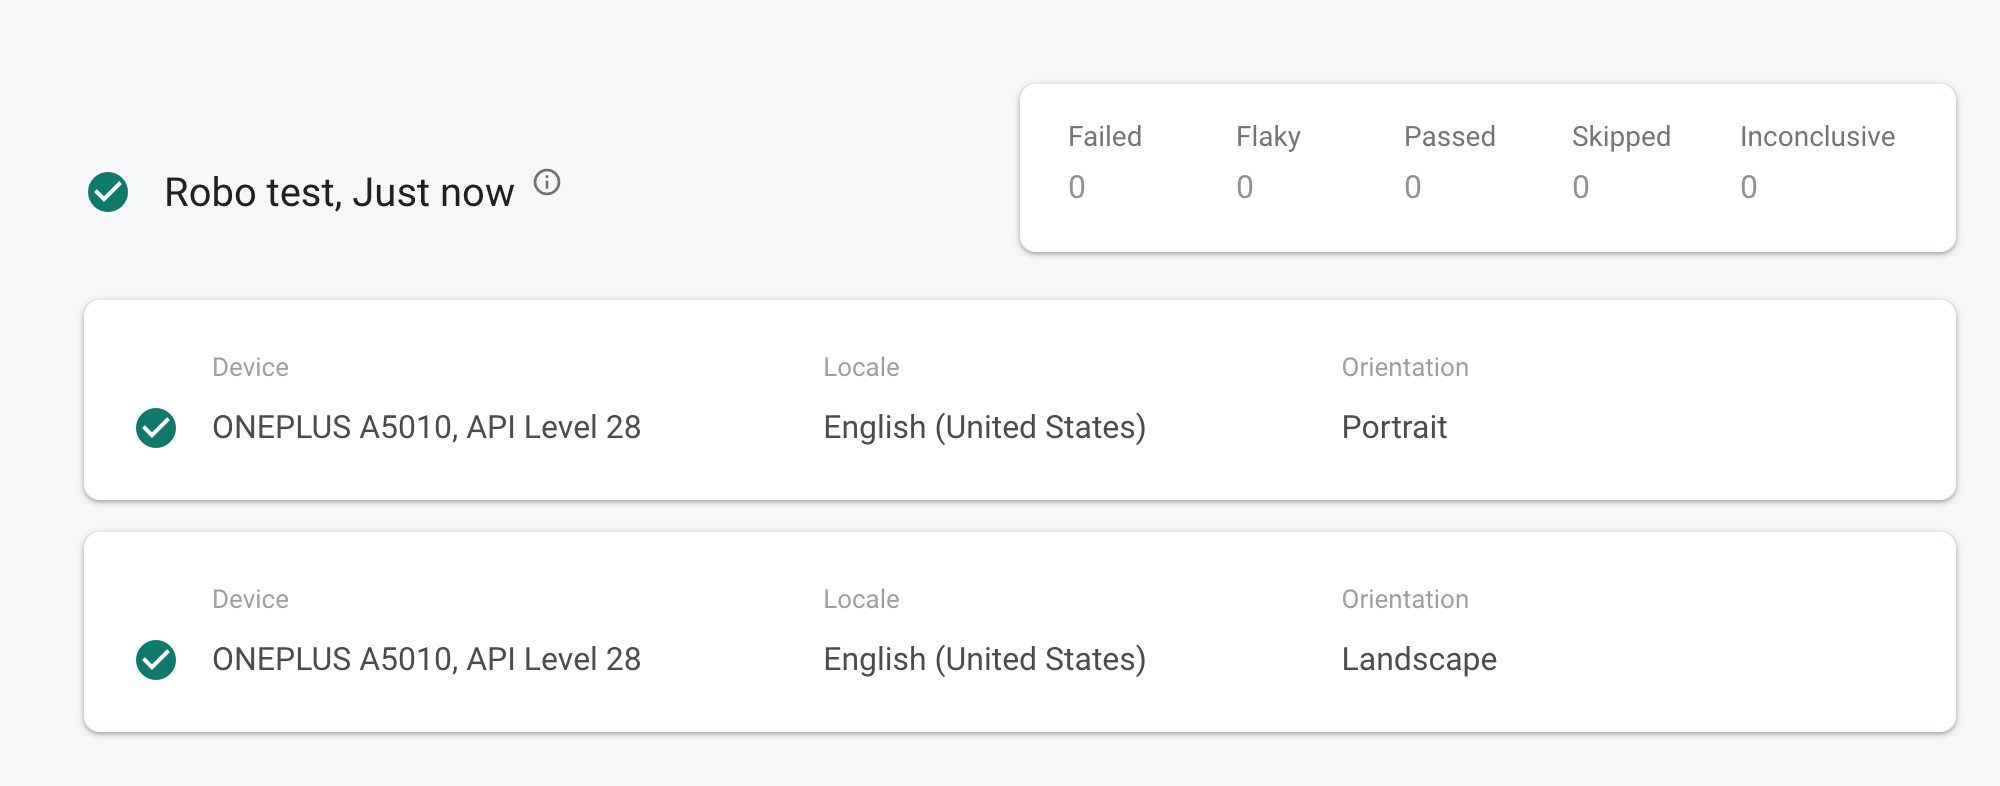
\includegraphics[width=150mm,scale=0.9]{./Images/testing/testing2.png}}
  \caption{Robo test}
\end{figure}